%!TEX root = ../../architekturdokumentation.tex
\chapter{Logische Architektur}


%!TEX root = ../../architekturdokumentation.tex
\section{Backend Architektur}
	Nachfolgend werden wichtige architektonische Klassen und deren Zusammenhang im Backend mittels Klassendiagrammen beschrieben.

	\subsection{Klassendiagramm}
	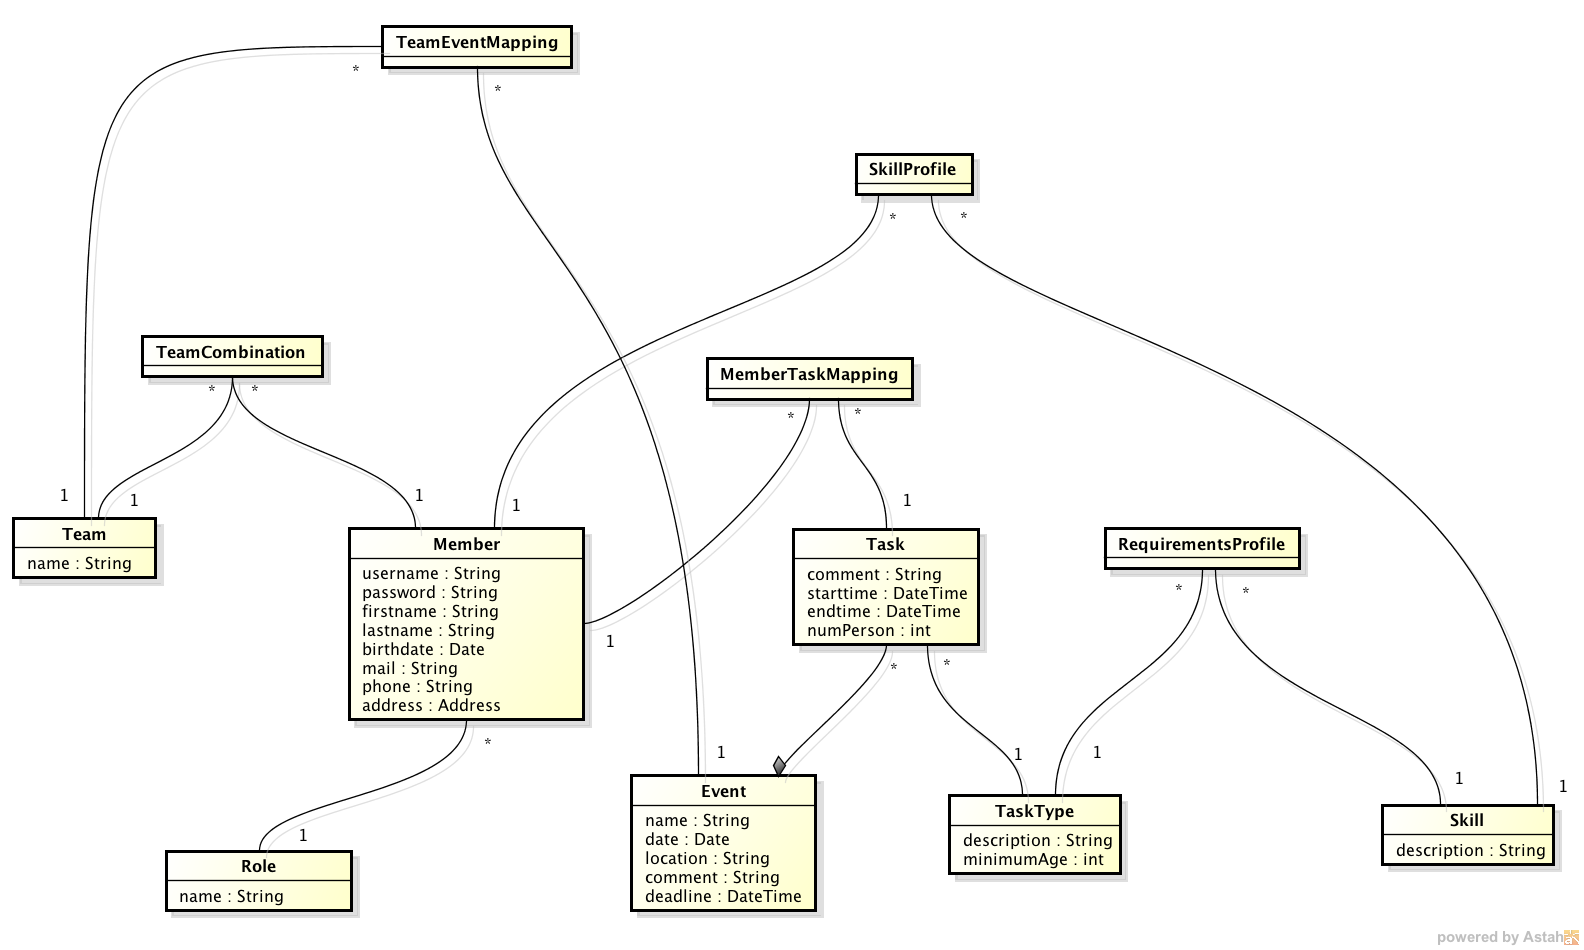
\includegraphics[width=\textwidth]{content/architekturdokumentation/images/datenmodell.png}
	
	\subsection{Typische Systemoperationen}

	\subsection{Wichtige Design Aspekte}
		\subsubsection{Model-View-Controller}
		Für die Presentationschicht setzen wir MVC ein, da ASP.NET eine gute Unterstützung für dieses Modell bietet. Auf alle Seiten wird mittels Controller zugegriffen. Die Views werden mithilfe der Razorsprache erstellt.


		\subsubsection{Entity Framework Code-First}
		Gemäss den Empfehlungen von Microsoft, soll für neue Projekte Code First eingesetzt werden. In diesem Konzept wird das Datenbankmodell direkt durch den C\# Code generiert. Dies bietet uns den Vorteil dass man nur noch mit C\# arbeiten muss.

\section{3-Tier-Architektur}
	Um eine möglichst hohe Abstraktion unseres Codes zu erhalten, haben wir uns für eine 3-Tier-Architektur entschieden, die unsere Applikation in die drei Schichten Web, Service und DataAccesLayer (Dal) unterteilt. Alle Datenbankspezifischen Operationen sollen im DAL vorgenommen werden. Alle Zugriffe aus dem Web sollen über die Web-Layer behandelt werden. Die Zugriffe auf externe Schnittstellen über den Service-Layer.
	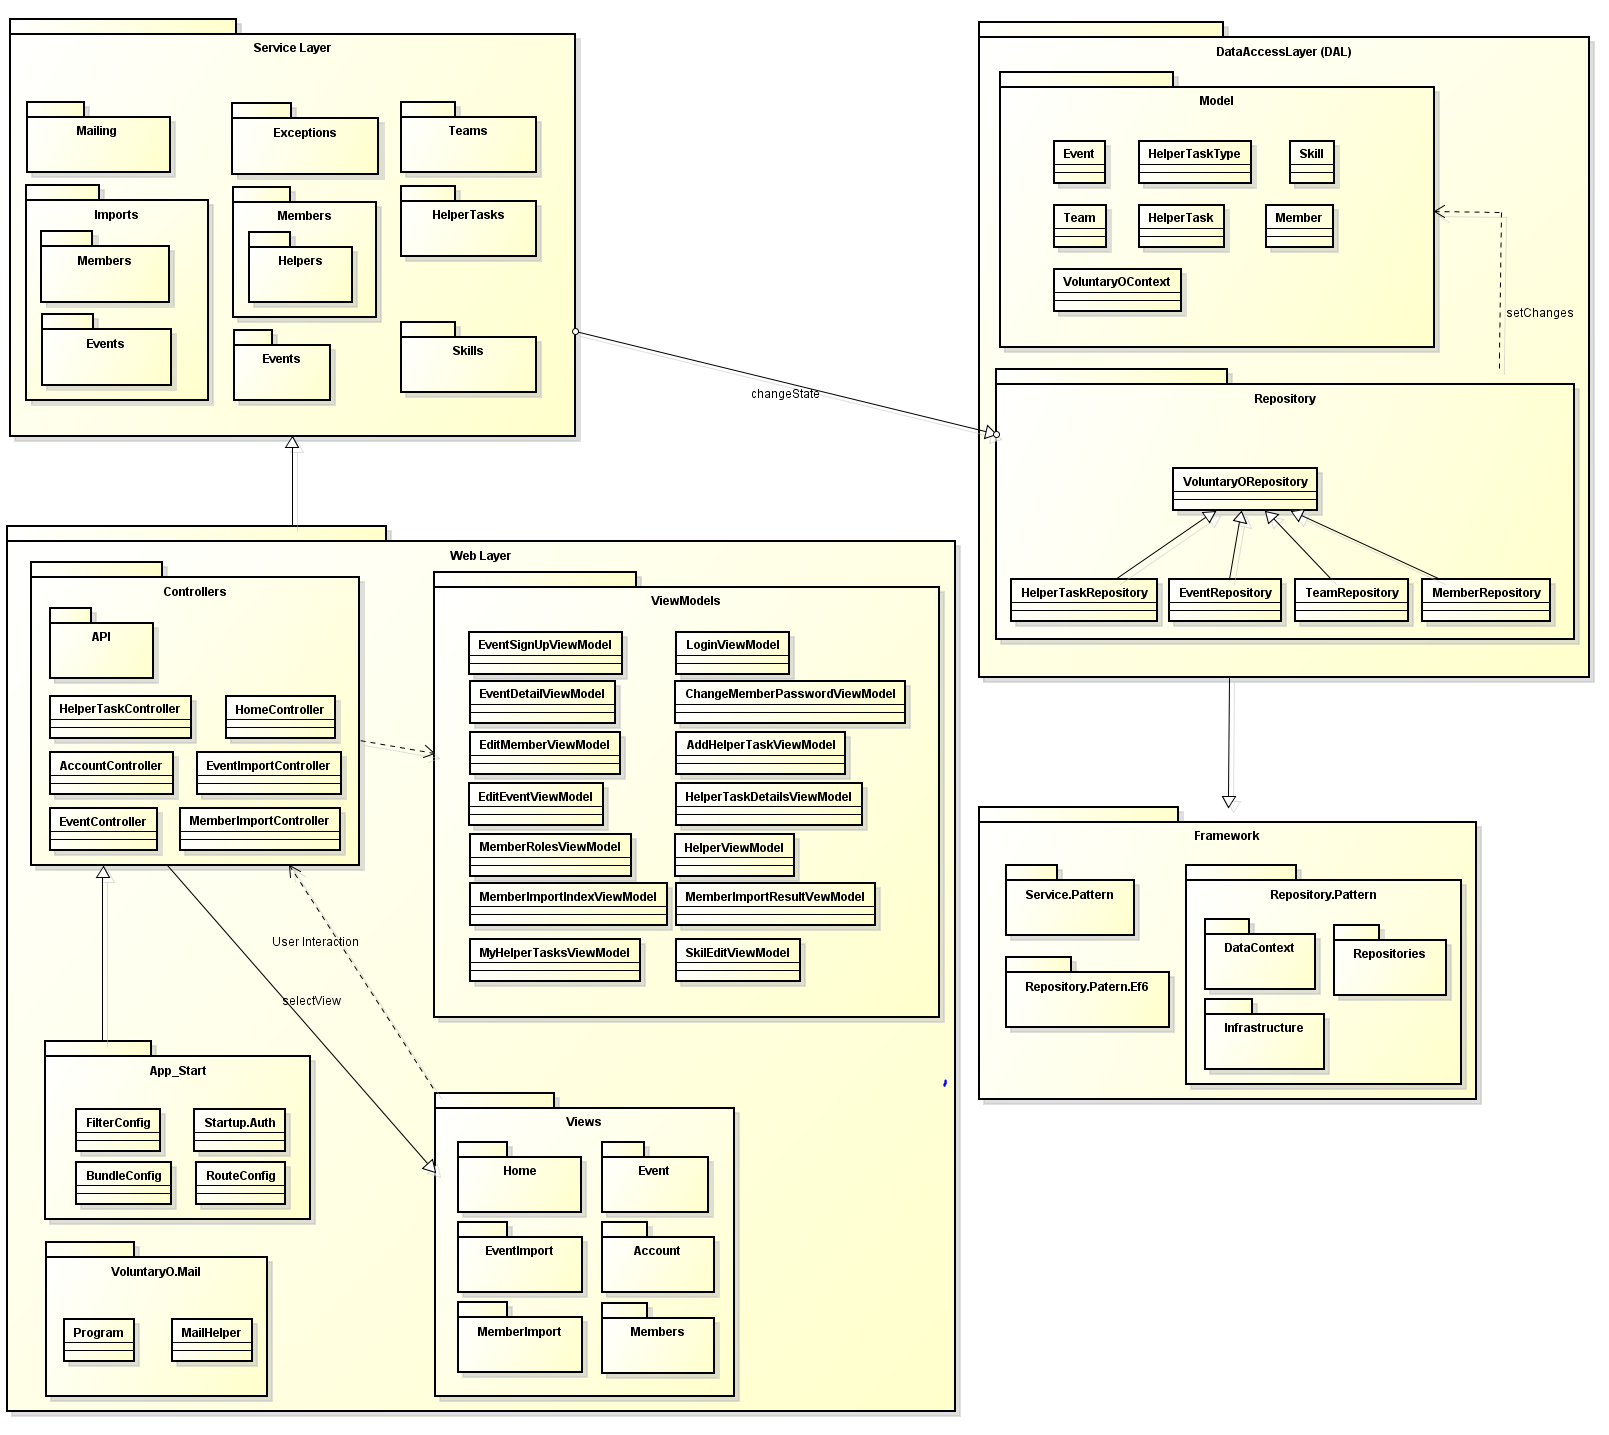
\includegraphics[width=\textwidth]{content/architekturdokumentation/images/LogischeArchitektur.png}

\section{VoluntaryO.Dal (Data Access Layer)}
    \begin{figure}[h]
  		\vspace{-5pt}
    	\centering
    	% VOLO-124
		% \includegraphics[width=\textwidth]{content/architekturdokumentation/images/domain.png}
  		\vspace{-25pt}
    	\caption{Domain in Subsystem VoluntaryO.Dal}
	\end{figure}
	Jede Model-Klasse implementiert die Schnittstelle \textit{IObjectState}, resp. leitet von der abstrakten Klasse \textit{Entity} ab.

	\subsection{Mapping}
	Das Mapping wird mit dem \textit{modelBuilder} des EF gesteuert. Bspw.
	\begin{lstlisting}[language=CSharp, caption=Mapping in VoluntaryoContext.cs, label=lst:mappingcontextcs, firstnumber=1]
// TeamEventMapping
modelBuilder.Entity<Team>()
    .HasMany(t => t.Events)
    .WithMany(e => e.Teams)
    .Map(mc =>
    {
        mc.MapLeftKey("TeamID");
        mc.MapRightKey("EventID");
        mc.ToTable("TeamEventMappings");
    });
    \end{lstlisting}

	\subsection{Vergleich für Objekte}
	Einzig für die Member-Klasse wurde die Vergleichsmethode (Equals) überschrieben. Folgende Attribute der Klasse sind relevant:
	\\\begin{itemize}
		\item \textit{UserName}
		\item \textit{Firstname}
		\item \textit{Lastname}
		\item \textit{Birthdate}
	\end{itemize}

	\subsection{Repository / Unit of Work Pattern}
	Generell wird das \href{https://genericunitofworkandrepositories.codeplex.com/}{\textit{Generic Unit of Work \& Repositories Framework}} befolgt um den Code Test- und Wartbar zu halten. Folgende Vorteile tun sich auf:
	\\\begin{itemize}	
		\item Austauschbarkeit ORM
		\item Testbarkeit
		\item Jeder Request hat eigene Unit of Work (siehe später Dependecy Injection)
		\item Reduktion der Datenbankabfragen, da nur noch über Unit of Work commited wird
		\item Generische Abfragen von Entitäten
	\end{itemize}
	Folgende Konventionen ergeben sich aus für das Projekt:
	\\\begin{itemize}
		\item Jede Entität implementiert \textit{IObjectState}
		\item Repository kann über \textit{partial Classes} erweitern werden
		\item Oder Repository Klassen implementieren \textit{IRepository} und erben von \textit{Repository}
	\end{itemize}

	\subsection{Unit Tests mit Effort}
	\href{https://effort.codeplex.com/}{\textit{Effort}} ist ein ADO.Net Provider und erstellt jeweils eine In-Memory Datenbank für das EF. Die temporäre Datenbank ermöglicht uns ein Testen des Codes, ohne Datenbankzugriffe zu mocken.
	\begin{lstlisting}[language=CSharp, caption=Verwendung Effort für Unit Tests in EffortTest.cs, label=lst:effortunittest, firstnumber=1]
		DbConnection Connection = DbConnectionFactory.CreateTransient();
		VoluntaryoContext VoluntaryoContext = new VoluntaryoContext(_Connection);
    \end{lstlisting}
    Den einzelnen Unit Tests steht so eine saubere und testbare Datenbank zur Verfügung.


\section{VoluntaryO.Service}



\section{VoluntaryO.Web}

	Die komplette Implementierung des Frontends befindet sich im Projekt Voluntary.Web. Folgend werden die Konzepte beschrieben, die wir zur Darstellung des Frontends verwenden.

	\subsection{View Model und Razor}
	Um die Websiten dynamisch darzustellen nutzen wir die ASP.NET Razor View Engine. Eine Razor-View ist immer mit einer Methode des Controllers verbunden. Das bedeutet auch, dass der Return-Wert der Methode sämtliche Daten mitliefern muss, die später in der View gebraucht werden. Da in einer View häufig mehr als nur ein standard Objekt aus dem Model gebraucht wird, haben viele Views ein Extra Viewmodel. Das bedeutet es wird extra eine Instanz eines speziell auf die View zugeschnittenen Objekt erstellt. Dieses View-Model enthält alle Referenzen auf andere Objekte, die innerhalb der View gebraucht werden.
	Durch den Einsatz des View-Model haben wir den Vorteil, dass pro View genau definiert ist, welche Daten wir brauchen. Der Zugriff auf das View-Model kann einfach getestet werden.
	Der Einsatz eines View-Models bietet aber auch einige Nachteile, beispielsweise werden manche Methoden redundant implementiert. Da wir die Implementation der Methoden aber sowieso auf die Service-Schicht abstrahiert haben, birgt dies für uns kein Problem.
	Da wir nicht durch das Model pro View eingeschränkt werden wollen bietet uns das View-Model den besten Dienst.

	\subsection{Bootstrap, CSS und JS}
	Das Front-End Framework, dass wir einsetzen ist Twitter Bootstrap. Zusätzlich verwenden wir ein verändertes CSS-File um nicht den typischen Bootstrap-Look zu erhalten.
	Zusätzlich setzen wir die Javascript-Library JQuery ein.
	ASP.NET bietet einen für die Einbindung von CSS- und JS-Files einen Bundle-Konfigurator an. So können CSS-Files oder JS-Files in Bundles gruppiert werden. Per View kann man dann genau definieren welche Bundles aktuell gebraucht werden. ASP.NET bindet einem dann automatisch die entsprechen Files in die HTML-Datei ein.
	Besonders nützlich ist hier, dass während der Entwicklungs-Phase die Files noch einzeln und noch nicht minifiziert übertragen werden. Sobald man die Applikation aber auf den Server deployed werden die Files automatisch in ein File gerendert und auch minifiziert, was für die Übertragungsgeschwindigkeit wichtig sein kann.
	Dabei wird pro Bundle ein File ausgeliefert, was besonders für das HTML-Caching wichtig ist.

	\subsection{AJAX und WebAPI}
	Unser Ziel ist es, dass unsere Applikation möglichst dynamisch sein soll. Dafür ist der Einsatz von asynchronen Request extrem wichtig. In unserer Applikationen sind mehrere verschiedene Implementationsarten dieses Konzeptes eingesetzt worden. Wenn möglich wurden die direkt von ASP.NET unterstützten Features genutzt. Hier wird über ein sogenanntes Ajax-Form in der Razor-Syntax ein AJAX Befehl konfiguriert. Als Return-Value wird hier ein Partial-View zurückgegeben. Dieser ersetzt dann ein bestehendes Partial-View.
	Besonders gut ist hier, dass unobstrusive-AJAX eingesetzt wird. Das bedeutet dieser Code würde auch funktionieren, wenn Javascript nicht aktiviert wäre.
	Für die komplexeren AJAX-Requests, die nicht mehr durch die ASP.NET Boardmittel gelöst werden können, haben wir ein REST Web-Api implementiert. Dieses API ermöglicht es durch AJAX-Request JSON Daten zurückzukriegen und diese dann dynamisch auf der Seite zu implementieren.
	Das Web-Api ist massgebend für die dynamik der Page.
